\subsection{Avant AIKON : le projet EnHerit}

\gls{enherit}\footcite{EnHeritEnhancingHeritage} est un projet ANR porté par l'Ecole nationale des ponts et chaussées qui s'est déroulé entre 2018 et 2023.

Ce projet a pour objectif d'isoler des \textit{patterns} récurrents dans plusieurs documents iconographiques pour tracer des liens entre ces derniers.

Les chercheurs du projet ont choisi de travailler sur un \textit{dataset} de 1587 œuvres attribuées à Jan Brueghel et son atelier. Contrairement à ce que nous pourrions penser, les œuvres d'art produites dans ce type de contexte ne sont pas toutes uniques. Il est fréquent que des croquis préliminaires et des études soient dupliquées et réutilisés sur d'autres œuvres. Cependant, reconnaître les motifs et faire des liens entre les différentes œuvres n'est pas une tâche évidente, notamment à cause de la diversité des techniques utilisées comme la peinture à l'huile, le pastel ou le dessin par exemple. A travers ce \textit{dataset}, l'équipe du projet \gls{enherit} cherche à extraire des \textit{patterns} récurrents et à réaliser des connexions visuelles entre les différentes œuvres de l'atelier de Jan Brueghel. Les outils développés à partir de ce \textit{dataset} permettent aux historiens de l'art de réaliser une tâche qu'auparavant ils accomplissaient à la main. En effet, ces avancées ont pour but de remplacer la collation manuelle des images durant laquelle les historiens de l'art traçaient à la main chaque motif pour ensuite les comparer. Dans le cas du \textit{dataset} de l'atelier de Jan Brueghel, cela représenterait plusieurs années de travail.

\begin{figure}[h]
	\centering
	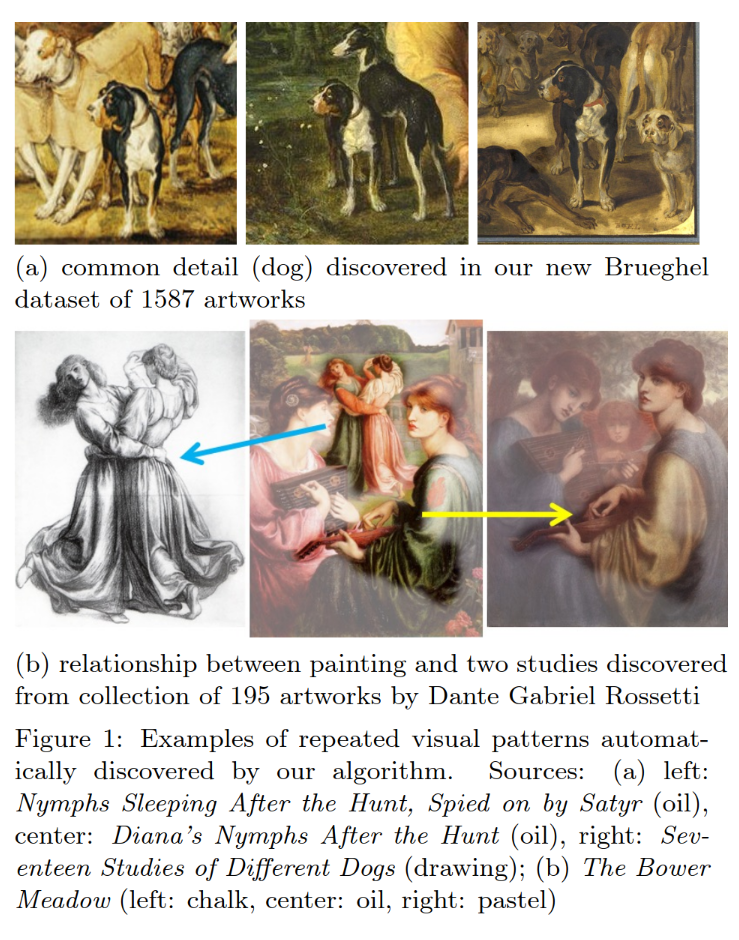
\includegraphics[width=0.7\linewidth]{images/exemples_patterns_enherit.png}
	\caption{Exemples de \textit{patterns} répétés dans plusieurs œuvre issues du data de Jan Brueghel \footcite{shenDiscoveringVisualPatterns2019}}
	\label{fig:exemples_patterns_repetes}
\end{figure}

Cependant, l'un des problèmes que nous pouvons rencontrer dans ce type de projet est l'annotation manuelle qui peut se révéler fastidieux pour les historiens de l'art. C'est pour cette raison, que les chercheurs du projet \gls{enherit} ont choisi d'utiliser l'apprentissage auto-supervisé aussi appelé \textit{self-supervised learning}\footcite{shenDiscoveringVisualPatterns2019}.
L'apprentissage auto-supervisé est \og une technique de \textit{machine learning} qui utilise l'apprentissage non-supervisé pour des tâches qui, habituellement, nécessitent un apprentissage supervisé \fg. Dans le cadre de l'apprentissage supervisé, il est nécessaire d'annoter les données au préalable tandis que dans l'apprentissage non supervisé, un algorithme les génère tout seul\footcite{QuestceQueLapprentissage2023}.
Pour effectuer cette tâche, il est nécessaire au préalable de réaliser un apprentissage des caractéristiques. Il faut d'abord échantillonner un \textit{patch} pour trouver des candidats. Ensuite, nous filtrons les faux positifs par le biais de la cohérence spatiale avant de mettre en place un apprentissage métrique avec des paires positives et négatives. C'est de cette manière que l'outil ArtMiner a été développé\footcite{ArtMiner}. Ce dernier est réutilisé par la suite par le projet \gls{vhs}. 
L'algorithme Segswap disponible dans l'application AIKON est également issu de ce projet.

A partir des avancées réalisées dans le cadre de \gls{enherit}, un autre projet est né : le projet AIKON.

\subsection{L'application AIKON}

AIKON est une application de recherche conçue pour permettre aux chercheurs en Sciences Humaines et Sociales d'exploiter des outils de computer vision afin d'analyser de vastes corpus de données historiques\footcite{aikonAikonplatformAikon2025}. 
Sa plateforme mais aussi les modèles d'intelligence artificielle disponibles dessus sont tous \textit{open source}. Cela signifie que n'importe qui peut accéder au code et utiliser l'application de manière gratuite. Elle est donc à la fois accessible à de gros projet mais aussi à des chercheurs qui l'utiliseraient pour des projets personnels. 
AIKON permet de décrire les sources historiques et analyser des corpus visuels en vue de leur potentielle édition\footcite{albouyAIKONComputerVision}.

Au delà des outils de \textit{computer vision} qu'elle propose, AIKON est aussi un excellent outils de gestion des sources numérisées. Elle permet de déposer des témoins numérisés dans différents format (jpg, pdf ou manifest IIIF) avec la possibilité de les transformer en manifest IIIF si ce n'est pas déjà fait. Il est aussi possible de décrire des \textit{witnesses} de manière précise en fournissant des métadonnées sur la cote, le lieu de conservation ou bien l'auteur. Il est également possible de créer des fiches pour des éléments comme les \textit{works} ou \textit{authors} par exemple qui pourront être réutilisés pour différents \textit{witnesses}.   --> déplacer dans 2.3 ???

Avant de faire subir des traitements aux witnesses, les chercheurs peuvent les organiser en ensembles cohérents notamment en \textit{series}.


\subsection{Le projet VHS}

\gls{vhs} est un projet qui a pour but de mettre en place une nouvelle approche de l'étude historiques du savoir scientifique en utilisant les outils numériques pour l'analyse d'image. Il rassemble trois équipes de recherche : l'équipe Digital Humanities de l'Institut des Sciences du Calcul et des Données de Sorbonne Université, l'équipe Monde Byzantin du laboratoire Orient et Méditerranée (UMR 8167) et l'équipe IMAGINE du Laboratoire d'informatique Gaspard Monge de l'Ecole nationale des Ponts et Chaussées\footcite{Presentation}.* Carnet Hypothèse VHS Il a permis de constituer un nouveau \textit{dataset} d'illustrations scientifiques du Moyen-Age et de l'époque moderne. Cela a permis d'extraire près de 235000 images à partir de 405000 pages du corpus. Suite à l'annotation manuelle des résultats d'extraction d'image, 8000 d'entre-elles ont été validées par des historiens\footcite{fouadComputerVisionHistorical2023}. Ce \textit{dataset} est composé de quatre corpus sélectionnés pour leur diversité en ce qui concerne leur thématique, leur époque et leur aire géographique. 
Nous avons d'abord le \textit{Physiologus} un texte rédigé vers le IIe siècle de notre ère à Alexandrie. Il est composé d'une centaine de manuscrits écrits en grec dont 13 d'entre eux sont illustrés. Ces derniers ont été réalisés entre le XIe et le XVIe siècle et ils ont été diffusés dans tout l'Occident chrétien. Nous avons pu extraire environ 680 images d'animaux, de plantes et de minéraux. 
Le deuxième corpus concerne le \textit{De materia medica} écrit vers 77 de notre ère par Dioscoride. Il est conservé dans 65 manuscrits grecs. 17 d'entre eux réalisées entre le VIe et le XVIe siècle sont illustrés d'environ 8340 images de plantes, d'animaux et de minéraux. 
Les deux derniers corpus contiennent des planches de \textit{l'Encyclopédie} de Diderot et d'Alembert publiées entre 1751 et 1772 mais aussi leurs sources et leur inclusion ultérieure dans d'autres encyclopédies. Les deux thèmes principaux de ces corpus sont l'histoire naturelle et les sciences mathématiques. 
Ainsi, nous retrouvons au sein du projet \gls{vhs} à la fois deux œuvres datant de l'Antiquité et ayant été diffusés durant tout le Moyen Age et l'époque moderne dans tout l'Occident mais aussi une œuvre plus tardive qu'est \textit{l'Encyclopédie} de Diderot et d'Alembert qui a également eu une grande influence notamment dans l'écriture d'encyclopédies postérieures\footcite{Corpus}.* VHS Hypothèses (corpus)



\subsection{Le projet EIDA}

\gls{eida} est un projet ANR PRC d'envergure internationale qui a pour but l'étude et l'analyse des diagrammes de tradition ptolémaïque dans un corpus de témoins allant du IXe siècle au XIXe siècle avec des sources en latin, hébreu, sanskrit, byzantin, perse, grec, chinois et arabe. Il rassemble deux équipes de recherche. Le laboratoire \gls{lte} de l'Observatoire de Paris s'occupe principalement de la partie histoire des sciences du projet tandis que l'équipe IMAGINE de l'Ecole nationale des Ponts et Chaussées gère la partie \textit{computer vision}\footcite{albouyAIKONComputerVision}. 

Le but du projet serait de développer des outils pour que les chercheurs puissent explorer, visualiser le corpus, communiquer les résultats lors de conférences et réaliser des éditions de diagrammes nativement numériques \footcite{Conference2023EIDA2023}.

Le projet encore en cours s'est déroulé en plusieurs étapes. La première concernait la constitution du corpus. Les chercheurs cherchent à étudier le diagramme sous un angle documentaire en tant que artefact et sous son angle épistémique en tant qu'outil de compréhension pour les acteurs historiques\footcite{Conference2023EIDA2023}.

Suite au développement des premiers outils numériques de la plateforme, il a été possible d'appliquer aux sources de premiers traitements automatiques. L'extraction puis la reconnaissance automatique de \textit{region pairs} et le calcul de similarité ont permis de distinguer les diagrammes en double et de les interpréter dans plusieurs traditions, œuvres et témoins\footcite{Conference2024Graphic2024}.

Les chercheurs ont pu réaliser de premières observations. Il se trouve que les diagrammes peuvent être regroupés en fonction de leurs similarités. Un diagramme peut être rattaché à une œuvre, à une thématique ou à une famille\footcite{Conference2025Long2025}. 

Les chercheurs se réunissent régulièrement pour mener une réflexion autour du projet lors de conférences et séminaires. 
 

Sur le long terme, le but du projet serait de mettre à disposition des chercheurs une interface utilisateur sur le modèle de celle de \gls{dishas}, un projet antérieur mené par l'Observatoire de Paris. \\

D'autres projets ont souhaiteraient utiliser AIKON à l'avenir pour traiter leurs sources. C'est le cas du projet ANR High Vision dont le but est d'étudier en s'aidant de la \textit{computer vision} des photographies de presse datant de la fin XIXe siècle au début du XXe siècle qui ont été numérisées en masse. * carnet hypthèse High Vision



 